\subsection{VCT regression}
\label{sec:result_VCT_regression}
Manoeuvring model tests are used to assess the physical correctness of the manoeuvring models. As a first step, total forces and moments from the model test are estimates with inverse dynamics (see \autoref{sec:inverse_dynamics}). These forces can be compared with corresponding forces predicted with the manoeuvring model. 
\autoref{fig:VCT_regression_ID} shows such a comparison for a zigzag20/20 model test and the VCT regressed Semi-empirical model. The top graph shows the rudder signal $\delta$ together with drift angle $\beta$ and yaw rate $r$. A comparison of sway force $Y_D$ and yawing moment $N_D$ are shown in the other two graphs. The forces and moments predicted with the Semi-empirical model are in reasonable agreement with the forces from the experiment. There are small deviations, where the model over predicts the forces and moments in the peaks -- in the ends of the counter rudder excitations. The predicted force signals seem to have the same general shape as the experimental forces, which implies that the model structure captures most of the essential physics involved in the experiment. The Semi-empirical model is therefore a good candidate to be used in the inverse dynamics regression (IDR) which is investigated in the next section.
\begin{figure}[h!]
    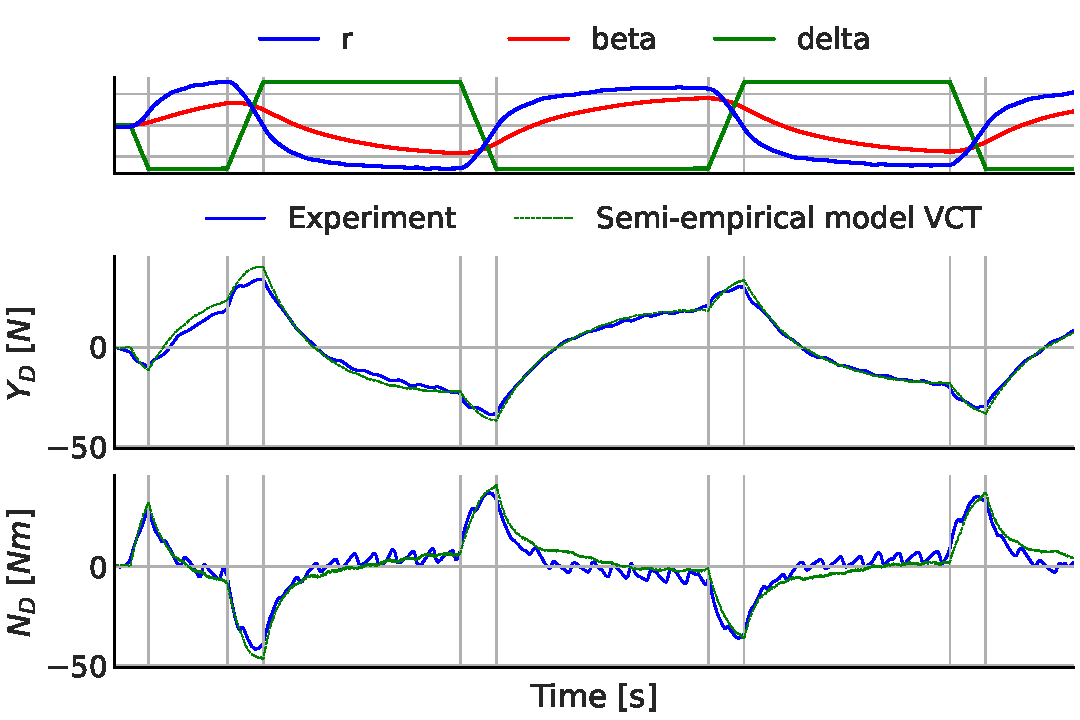
\includegraphics[width=\textwidth]{figures/result_VCT_regression.VCT_regression_ID.pdf}
    \caption{Comparison of the total forces on the ship predicted with the Semi-empirical model from the VCT regression and corresponding values from a zigzag20/20 test estimated with inverse dynamics.}
    \label{fig:VCT_regression_ID}
\end{figure}
